\chapter{Methods} \label{chapter:methods}
The research project consists of two major phases. Phase 1 is all about analysis: Determining user requirements and finding out what goals these users are trying to achieve by using the software. Phase 2 is about design and user testing. Based on the analyses and the results of the literature study a first prototype is designed and tested. The insights inform the design of the second iteration, which is then tested again in a more thorough way and with more users. This last study not only assures that the implemented changes had a positive impact, but also verifies that all user requirements have been met and that the software allows users to perform all necessary tasks.

\section{Phase 1: Analysis}
The first phase of the project consisted of user research, which established requirements and shed more light on the users' needs. The research served as the basis for designing the first prototype, as described later on, and was also used at the end of the project to determine whether the newly designed software met its purpose. 

\subsection{User Requirements Analysis}
In addition to segmenting the different users into groups requirements were gathered. Since most users are full-time employees at Babbel they were easily accessible. Because of this, requirements were gathered through observational field visits and interviews as proposed by Goodman et al. \cite{goodman_observing_2012}. The observations were particularly fruitful, as users were using an existing content authoring tool already. This helped most of them verbalize what they did not like about it. During the observations the author stayed in the background and only inquired about details of a user's behaviour every now and then. In general, users were left alone and just watched. The field visits were arranged in advance to make sure that users had enough time and were actually using the existing tool at that moment. Each session lasted about 20-30 minutes and was followed by a short interview or open discussion. The author made sure that what he had observed was not based on a wrong understanding and the users could raise concerns or point out especially annoying design flaws. At large, the atmosphere was kept informal so that users could behave natural and did not feel like being part of an artificial situation. The field visits resulted in a long list of requirements phrased as user stories. The stories were composed in a simple structure (see below) as suggested by Cohn \cite{_user_2004}. Terms in angle brackets need to be replaced and square brackets signify an optional section. The stories were ranked by type (functional or quality requirement) and importance. They can be found in Chapter \ref{chapter:user-research}.

\begin{figure}[h!]
\centering
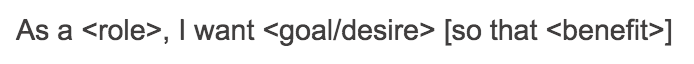
\includegraphics[width=9cm]{user-story-template}
\caption{User Story Template by Mike Cohn}
\label{fig:user-story-template}
\end{figure}

\subsection{Task Analysis}
There are many different ways of analyzing tasks and structuring them in a coherent way. All task analyses are in some way focused on decomposing a task into its constituting parts. The result is often some kind of diagram that visualizes the hierarchy or flow that is inherent to the task. 

For this project, a method called \ac{HTA} was used \cite{hornsby_hierarchical_2010}. It is a simple but effective method for studying work processes and was developed in the 1960s by two psychologists, Annett and Duncan \cite{shepherd_hierarchial_2000}. Their aim was to understand the purpose of work by looking at human activity within organisations and systems. HTA, in the tradition of systems thinking, regards work as a complex system consisting of  interacting sub-systems, which can be machines and humans \cite{shepherd_hierarchial_2000}. These sub-systems interact by means of input and output. The interplay is constantly adjusted through feedback mechanisms, which allow a human operator, to adapt his or her behaviour. 

Based on the analysis, diagrams were created, each of which represents a high-level task that is decomposed into sub-tasks. Each diagram provides an overview of the order in which tasks are performed as well as the mental processes behind them. The diagrams together with a short description of each task can be found in Chapter \ref{chapter:user-research}.

%The complex system examined in this particular case was the process of creating new learning content.

%The HTA described in this section is aimed at identifying tasks that could benefit from the implementation of a version control system. Moreover, the analysis helps visualize how tasks, performed by different user groups, overlap. This could support the design of an interface that facilitates and simplifies collaboration. 

\section{Phase 2: Iterative Design \& Usability Testing}
The second phase consisted of designing and iteratively testing the new interface. The first prototype was based on the insights gained through task and requirements analysis as well as the literature study. It served as a first starting point for discovering usability issues of the version control features of the system.

%This prototype was tested in a scenario-based usability study, which lay focus on the newly designed version control features. 

%maybe mention that research didn't start from scratch - there is other research that has proven version control can be valuable outside of programming - that's why I didn't start with exploratory resarch but with a summative tet 

\subsection{First Study}
% I dont like this paragraph
As a means of detecting usability problems early on the first study was conducted with a semi-interactive prototype that was based on simple graphical layouts. The prototype was mostly black and white and only those parts that were actually needed for the user tests were interactive. This meant that designing the prototype did not take a lot of time and subsequent modifications (i.e. after a design feedback round) could be realized quickly as well. 

The sessions were scenario-based, which means that participants had to perform a number of tasks which reflected their everyday work. This put more emphasis on the actual behaviour of users instead of opinions and attitudes and allowed the test moderator to stay in the background. This method is often referred to as \textit{assessment} or \textit{summative study} \cite{rubin_handbook_2008} \cite{goodman_observing_2012}. These kind of studies can yield more honest results because the method involves less interference than for example exploratory tests. The number of participants was kept rather small, informed by Nielsen's insight that 5 users are sufficient to find 85\% of the usability problems if the user group is somewhat uniform \cite{nielsen_why_2000}. 

Additionally, a few quantitative metrics were taken in order to support the results of the observations. Among them task completion rate, time for task completion and error rate. Because the sample size is somewhat small these metrics can rarely deliver statistically significant results, but they can serve as an indicator of potential problem areas that should be investigated further. How these metrics were measured is described in more detail in Chapter \ref{chapter:first-iteration}. 

% what is said?
% first paragraph:  prototype (needs work)
% second paragraph: type of study
% third paragraph: quantitative metrics
% fourth paragraph: write about the goals of the study?

% talk about kind of users
% which scenarios?
% or is this part of the subsequent chapters?

%This allows the test-moderator to  

%The goal was to eliminate the most severe problems before implementing them.  


%The goal of the first usability study was to detect severe problems before starting to implement any of the features.  

%The prototype was tested with a handful of users to detect usability problems early on. During this first assessment test, described in more detail 

\subsection{Focus Group}
All participants of the first usability study were also part of a subsequent focus group. The group meeting served as a platform for discussing concerns and the impressions regarding the novel version control features that users were exposed to during the testing sessions. Furthermore, the goal was to identify potential stumble stones in regards to the version control terminology. The terminology used by Git and other version control systems is often rather technical and not necessarily self-explanatory. But the aim is to make the system easy to learn for a non-technical user group as well.

% this paragraph was taken from the research proposal!!
Focus groups are particularly suitable for the early stages of a project. They can be an efficient means of gathering feedback in a short time-frame, because they involve more than one user at a time \cite{rubin_handbook_2008} \cite{goodman_observing_2012}. When conducting focus groups researchers need to be aware of the fundamental difference between what people say and what they do. Only because a participant claims that she likes a product, does not mean that she will actually use it \cite{goodman_observing_2012}. Therefore the outcome of the group should be put into perspective and not applied literally. Furthermore, the results of focus groups should be taken with a grain of salt, due to their small sample sizes. Nevertheless, the outcome can serve as a basis for further research \cite{goodman_observing_2012}. 

% this paragraph was taken from the research proposal!!
% maybe this should be rather part of the actual focus group section
%At the start of the focus group the test moderator explained the purpose of the meeting. Then, the participants were introduced to the version control features that will be exposed in the content authoring tool. These are only about five to six major features. Afterwards, the group will have a discussion on each of these features and whether it needs renaming. If the group comes up with more suitable names for  certain features, everyone is asked to write down his favorite terms on a piece of paper and prioritize them. This is done in order to mitigate social influences by people who are good at phrasing their strong opinions \cite{goodman_observing_2012}. At the end of the meeting there should be a list of proposed names for each term that needs to be renamed. The whole focus group session should not last longer than 1 1/2 hours.

\subsection{Second Study}
The second and final usability study was based on a functional web-based prototype. This prototype contained a number of changes that were made as a result of the findings of the first user study and the focus group. Most notably, the main navigation had changed as well as the way content was represented. Furthermore, a series of severe usability issues had been fixed, mostly related to the version control features of the system. On top of that, some of the main features were renamed, which had been identified as problematic during the focus group meeting. \textit{Branches} were now called \textit{working copies} and \textit{pull request} was changed into a more descriptive \textit{merge request}.

The main goal of this study was to verify whether the introduced changes had a positive impact on the user experience. Hence the name verification or validation study \cite{goodman_observing_2012} \cite{rubin_handbook_2008}.
For this reason, the setup of the study was similar to the first study, which made comparing the results easier. The web-based prototype, which covered a lot of functionality, allowed the moderator to stay in the background so that users could freely interact with the system. This proved to be quite successful in that a lot of new issues were found that had not been discovered during the first study.  

Besides validating the changes the study was also aimed at confirming that the user requirements specified during the start of the project were met. This was done by simply observing whether users were able to perform the desired tasks. Furthermore, a post-study usability questionnaire was used that measured the perceived usability of the system. This helped to identify weak spots and potential areas that would need more attention in the future. 

% new prototype / changes
% talk about goals: 
% prove whether changes that have been made were positive. 
% check whether user requirements have been met
% establish standards for the future (PSSUQ)

% short summary of method, verification/validation
% similar tasks to round 1

\section{Summary}
This chapter described the theoretical basis of the methodology used throughout this research project. The design of the user studies and the procedure during the sessions is described in more detail in Chapters \ref{chapter:first-iteration} and \ref{chapter:second-iteration}. The following chapter will introduce the reader to other research that has been done in the field of version control systems, with a special attention to systems applied outside of the programming realm. The remaining project will build upon this insights and the first prototype was heavily influenced by these findings described in the next chapter. 


%The research project will be divided into two major phases. Phase one will be all about the user and finding out who the user actually is and what kind of goals he or she tries to achieve. For this purpose a bunch of popular user-centered design methods will be used, such as personas, task and requirement analyses and a focus group \cite{mao_state_2005}. 
%During the second phase, the insights gained through the different analyses will be used to create meaningful prototypes. The first prototype will be a static representation of the interface, which can be tested in an exploratory study \cite{rubin_handbook_2008}. The idea is to start with a prototype that maps Git's functionality more or less 1:1 and then see which concepts the users are struggling with the most and then find suitable solutions to that during the design of the next prototype. For the first prototype some inspiration will be obtained by existing GUIs for Git \cite{_git_????}.

%The results of the first user tests will inform the design of a second prototype. This prototype will incorporate interface solutions to the problems users encountered during the first user tests. The second prototype will be interactive so that it can be tested with less interference by the moderator. The hope is that a task-based assessment will yield more genuine results than the exploratory study, especially regarding details of the interface and certain micro-interactions.

%Depending on how well the prototype was received during the assessment a third iteration will be done in which flaws that were encountered are eliminated. This prototype will then be tested once again, with more or less the same setup and methodology.